% Report-TheoreticalCalculations.tex
% Simon Hulse
% simonhulse@protonmail.com
% Last Edited: Wed 27 Nov 2024 02:54:44 PM EST

% !TeX root = ./Report-Body.tex
\allowdisplaybreaks
\chapter{Theoretical Calculations}
The simulate NMR experiments, it will be necessary to determine the relaxation rates of all coherences that exist. For an I$_3$S spin system, this requires determining all the matrix elements, $\Gamma_{rs}$, of the $256 \times 256$ relaxation superoperator. These elements will give great insight into how well different NMR experiments will perform. As a step towards achieving this, a python programme was developed from code written within the Baldwin group, in order to implement the relaxation models presented in Section \ref{RelaxModels}. This script produces symbolic rate expressions as an output. For numerical considerations, a programme able to parse the symbolic outputs was created for this thesis. Explicit examples of calculations using these scripts are presented below. Highly detailed insights can be made about relaxation phenomena in I$_3$S spin-systems as a result.
\section{Relaxation Rates Considered} \label{RatesConsidered}
A selection of relaxation rate calculations utilising the models established are presented in the subsequent sections of this chapter. The rates chosen were those of S-spin single-quantum coherences. These coherences correspond to the product operators $\hat{S}^{\alpha \alpha \alpha +}$, $\hat{S}^{\alpha \alpha \beta +}$, $\hat{S}^{\alpha \beta \beta +}$, and $\hat{S}^{\beta \beta \beta +}$, whose rates are given by $\Gamma_{2,\text{C}}^{i}$, where $i \in \{\alpha \alpha \alpha, \alpha \alpha \beta, \alpha \beta \beta, \beta \beta \beta\}$. These are responsible for the observable signal in $^{13}$C NMR experiments, giving rise to a quartet peak structure, Figure \ref{CQuart}. Relaxation rates of these coherences can be determined rather easily experimentally, making it possible to assess the effectiveness of our relaxation models. Table \ref{Operators} provides explicit definitions of the relevant operators using the single-element basis. All relaxation rates considered are auto-relaxation rates, corresponding to diagonal elements of the relaxation super operator (i.e. $\Gamma_{r,r}$, where $r$ is one of the product operators listed in Table \ref{Operators}).
\begin{table}[]
\centering
\begin{tabular}{l|l}
Operator                           & Definition                                                                                                                                                                                                        \\ \hline
$\hat{S}^{\alpha \alpha \alpha +}$ & $\hat{I}_1^{\alpha} \hat{I}_2^{\alpha} \hat{I}_3^{\alpha} \hat{S}^{+}$                                                                                                                                            \\
$\hat{S}^{\alpha \alpha \beta +}$  & $\hat{I}_1^{\alpha} \hat{I}_2^{\alpha} \hat{I}_3^{\beta} \hat{S}^{+} + \hat{I}_1^{\alpha} \hat{I}_2^{\beta} \hat{I}_3^{\alpha} \hat{S}^{+} + \hat{I}_1^{\beta} \hat{I}_2^{\alpha} \hat{I}_3^{\alpha} \hat{S}^{+}$ \\
$\hat{S}^{\alpha \beta \beta +}$   & $\hat{I}_1^{\alpha} \hat{I}_2^{\beta} \hat{I}_3^{\beta} \hat{S}^{+} + \hat{I}_1^{\beta} \hat{I}_2^{\alpha} \hat{I}_3^{\beta} \hat{S}^{+} + \hat{I}_1^{\beta} \hat{I}_2^{\beta} \hat{I}_3^{\alpha} \hat{S}^{+}$    \\
$\hat{S}^{\beta \beta \beta +}$    & $\hat{I}_1^{\beta} \hat{I}_2^{\beta} \hat{I}_3^{\beta} \hat{S}^{+}$
\end{tabular}
\caption{Definitions of product operators which describe the S-spin single quantum coherences.}
\label{Operators}
\end{table}
\section{$^{13}$C Transverse Rates in a Methyl Moiety}
A significant amount of literature exists describing methyl relaxation rates, primarily due to the emergence of methyl-TROSY as a well established technique for studying high mass biomolecules. Expressions describing $^{13}$C transverse relaxation rates, $\Gamma_{2,\text{C}}^{i}$, have been presented previously in the literature, using different assumptions. A couple of these descriptions are now outlined, before we extend the treatment.
\begin{figure}
\centering
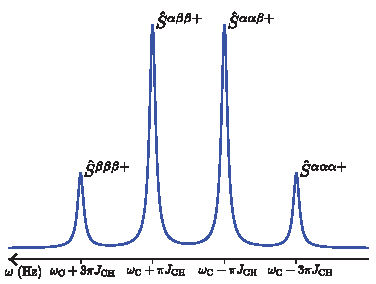
\includegraphics[scale=1.2]{./Figures/SimonsFigs/13CQuartet.pdf}
\caption{A simulated 1D $^{13}$C spectrum of a methyl moiety. A quartet of peaks are present, as a result of scalar coupling between the $^{13}$C nucleus and the $^{1}$H nuclei. The four peaks appear at frequencies $\omega_{\text{C}} - 3 \pi J_{\text{CH}}$, $\omega_{\text{C}} - \pi J_{\text{CH}}$, $\omega_{\text{C}} + \pi J_{\text{CH}}$, and $\omega_{\text{C}} + 3 \pi J_{\text{CH}}$, respectively, where $\omega_{\text{C}}$ is the resonance frequency of the $^{13}$C nucleus. Each peak is labelled by the product operator that corresponds to the signal it derives from.}
\label{CQuart}
\end{figure}
\subsection{Previous Accounts} \label{PreviousModels}
\subsubsection{Ollerenshaw et al., 2003}
In a paper illustrating the theoretical underpinning of methyl-TROSY, Ollerenshaw et al. presented remarkably simple expressions of the rates \cite{RN17}. Only dipolar interactions were considered. The methyl moiety's rotational motional motion about its C$_3$ axis was assumed to be infinitely fast. On top of what is presented in Section \ref{MethylRot}, an additional type of motion was included - that of the methyl symmetry axis. In Chapter 2, the motion of the symmetry axis is assumed to be perfectly correlated with the rest of the molecule. The possibility of this not being the case is approximated by a model-free approach, first described by Lipari and Szabo\cite{RN31}. Moreover, the macromolecular limit was invoked, in which it is assumed that $\omega_{\text{S}} \tau_{\text{c}} \gg 1$, where $\omega_{\text{S}}$ corresponds to the $^{13}$C Larmor frequency. In this limit, all spectral density terms for which $\omega \neq 0$ are negligibly small, and thus do not contribute to the rate expression. A term accounting for dipolar interactions with external protons was also included. NMR spectra are conventionally run on samples with high levels of deuteration in order to reduce such external interactions\footnote{Incorporation of deuterium into the sample reduces external dipolar interactions, on account of the smaller gyromagnetic ratio of deuterium, relative to proton ($\gamma_{\text{H}} \approx 6 \gamma_{\text{D}}$)}. Labelling strategies specific to the methyl-TROSY technique have been developed with this intention\cite{RN45}. Despite this, external dipolar interactions can still a have marked impact on relaxation rates, such that a full-scale calculation should include them.
\subsubsection{Hansen et al., 2009}
Less drastic approximations were presented by Hansen et al.\cite{RN4} As well as dipolar interactions, the CSA of the $^{13}$C nucleus was included as a mechanism able to induce relaxation. The Woessner Model, described in Chapter 2, was invoked to describe methyl rotation. Spectral density terms, $J\left(\tau_{\text{c}}, \omega\right)$\footnote{These spectral densities arise when $k_{\text{DW}} = 0$} with $\omega = \omega_{\text{S}}$ were included along as those with $\omega = 0$. It was again assumed that methyl rotation is rapid relative to the global motion of the molecule, meaning  $\tau_{\text{c}} \gg \tau_{\text{m}}$. In this limit, spectral density terms, $J\left(\frac{\tau_{\text{c}} \tau_{\text{m}}}{\tau_{\text{m}} + \tau_{\text{c}} k_{\text{DW}}^2}, \omega_{k,n_2}\right)$, for which $k_{\text{DW}} \neq 0$, reduce to $\frac{\tau_{\text{m}}}{k_{\text{DW}}^2} = \tau_{\text{m}}$.\\
To account for external interactions from remote protons, an additional term, $\frac{3}{2} \Gamma_{\text{sel}}$, was included, where $\Gamma_{\text{sel}} = \Gamma_{1,\text{H}}^{zz} - \Gamma_{1,\text{H}}^{z}$. $\Gamma_{1,\text{H}}^{z}$ and $\Gamma_{1,\text{H}}^{zz}$ are the auto-relaxation rates of the operators $2\hat{I}_z\hat{S}_z$ and $4\hat{I}_z\hat{I}_z\hat{S}_z$ respectively\footnote{$2\hat{I}_z\hat{S}_z = 2\hat{I}_{1z}\hat{S}_z + 2\hat{I}_{2z}\hat{S}_z + 2\hat{I}_{3z}\hat{S}_z$, and $4\hat{I}_z\hat{I}_z\hat{S}_z = 4\hat{I}_{1z}\hat{I}_{2z}\hat{S}_z+ 4\hat{I}_{1z}\hat{I}_{3z}\hat{S}_z + 4\hat{I}_{2z}\hat{I}_{3z}\hat{S}_z$}. This term stems from methyl proton longitudinal relaxation, driven by dipolar couplings with external protons. Such interactions are able to 'flip' the spin state of the external protons, and leads to an additional source of relaxation in the methyl moiety. Explicit expressions of $\Gamma_{1,\text{H}}^{z}$ and $\Gamma_{1,\text{H}}^{zz}$ were not presented by Hansen et al., though $\Gamma_{1,\text{H}}^{zz} - \Gamma_{1,\text{H}}^{z}$ was said to scale with $J(\tau_{\text{c}},0)$ in the macromolecular limit.  The desired term was obtained by using our result, and invoking the macromolecular limit.
\subsection{Comparison of the Models}
The accounts in Section \ref{PreviousModels} were compared with the spherical isotropic, Woessner and diffusive models presented in Chapter 2. This was done by assuming a $^{13}$C$^{1}$H$_{3}$ moiety, with a perfect tetrahedral geometry, such that the angle $\beta$ between the threefold rotation axis and the C-H bond vectors is $\cos^{-1}(-\frac{1}{3}) \approx \ang{109.47}$. Dipolar interactions with spins external to the methyl group were accounted for by assuming a single external proton was present, at an average distance of $\num{3} \si{\angstrom}$ from the methyl protons. The other parameters of relevance are stated in the caption of Figure \ref{CH3Models}. Explicit expressions derived from all relaxation models are presented in Appendix C. The angles of rotations applied to each tensor, to bring them into the molecular frame, are given in Table \ref{tab3.1}.\\
\begin{table}[]
\centering
\begin{tabular}{l|l}
Interaction tensor & $(\alpha, \beta)$           \\ \hline
$d_{\text{IS}} (1)$                              & $(\ang{0}, \ang{109.47})$   \\
$d_{\text{IS}} (2)$                              & $(\ang{120}, \ang{109.47})$ \\
$d_{\text{IS}} (3)$                              & $(\ang{240}, \ang{109.47})$ \\
$d_{\text{II}} (1)$                              & $(\ang{90}, \ang{270})$     \\
$d_{\text{II}} (2)$                              & $(\ang{90}, \ang{210})$     \\
$d_{\text{II}} (3)$                              & $(\ang{90}, \ang{150})$     \\
$c_{\text{S}}$                                   & $(\ang{0}, \ang{0})$        \\
$c_{\text{I}} (1)$                               & $(\ang{0}, \ang{109.47})$   \\
$c_{\text{I}} (2)$                               & $(\ang{120}, \ang{109.47})$ \\
$c_{\text{I}} (3)$                               & $(\ang{240}, \ang{109.47})$
\end{tabular}
\caption{The angles characterising the rotations of all interaction tensors into the Molecular frame.}
\label{tab3.1}
\end{table}
\begin{figure}
\centering
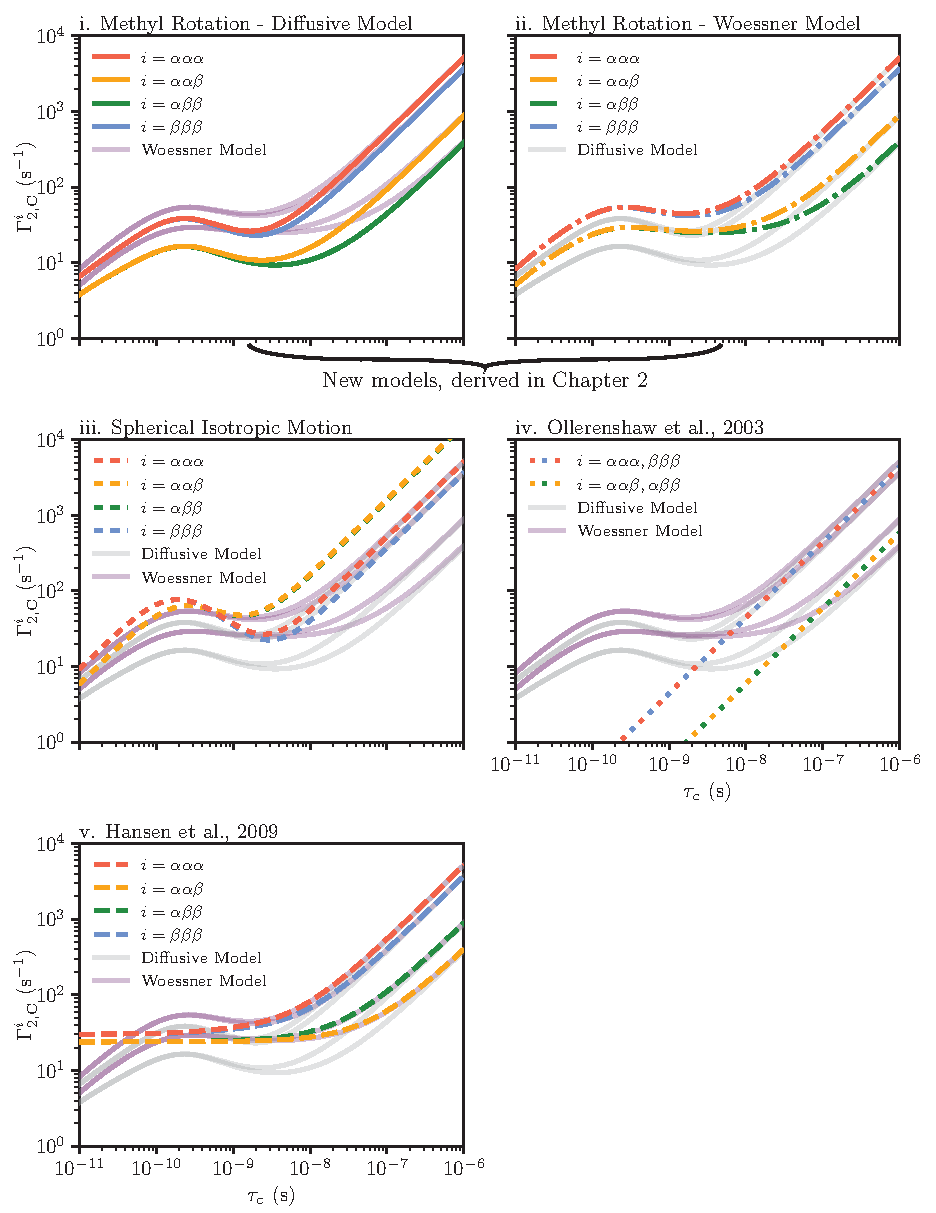
\includegraphics[scale=1]{./Figures/SimonsFigs/CH3models.pdf}
\caption{%
Plots of relaxation rate versus global tumbling correlation time,
$\tau_{\text{c}}$, for various I$_3$S relaxation models.
Parameters used: $B_0 = \num{14.1} \si{\tesla}$,
corresponding to a $\num{600} \si{\mega\myhertz}$ spectrometer,
$\gamma_{\text{S}} = \num{67.283e6} \si{\radian\per\second\per\tesla}$,
$\gamma_{\text{I}} = \num{267.513e6} \si{\radian\per\second\per\tesla}$,
$r_{\text{IS}} = r_{\text{II}} = \num{1.09} \si{\angstrom}$,
$\theta = \ang{109.47}$,
$\tau_{\text{m}} = \num{50} \si{\pico\second}$,
$\Delta \sigma_{\text{S}} = 20 \text{ppm}$,
$\Delta \sigma_{\text{I}} = 1 \text{ppm}$,
$S_{\text{axis}} = 1$ (this is described in Appendix D).
All plots have the results of the diffusive and Woessner model calculations
superimposed, for easy comparison.
}
\label{CH3Models}
\end{figure}
In Figure \ref{CH3Models}, plots ii., and v. show very good agreement for large values of $\tau_{\text{c}}$. This is exactly what is expected, since the both sets of expressions for the rates were derived using the Woessner model, but Hansen et al. apply the macromolecular limit. There are relatively marked differences in behaviour between the Woessner model (plot ii.) and the diffusive model (plot i.) when considering more rapid tumbling (smaller $\tau_{\text{c}}$ values). The trend for a decrease in rates with increasing $\tau_{\text{c}}$ in the region of $\tau_{\text{c}} \approx \num{e-9} \si{\second}$ is not something that was anticipated, and its origin is discussed below. The result of Ollerenshaw et al. resembles plots i., ii., and v. somewhat in the macromolecular limit. However, inclusion of the $^{13}$C CSA causes the rates of the other methyl rotation models to deviate from this model. The plots suggest that the carbon CSA has a noticeable, but non-dominating impact on the rates in the macromolecular limit.\\
It is clear that the spherical isotropic model in iii. is inappropriate, primarily as there is a gross overestimation of the inner line ($\alpha \alpha \beta$ and $\alpha \beta \beta$) relaxation rates, relative to the models that incorporate methyl rotation.
\subsection{Investigating Individual Contributions to the Rates}
The complete set of rate expressions derived are given in Appendix D, however in order to gain a more in-depth understanding of the form of the plots in Figure \ref{CH3Models}, rate of one specific line in the quartet: $\alpha \alpha \alpha$ (red) was considered in detail. Despite the very large number of terms that feature in the rate expressions, only a few terms tend to contribute significantly with any given value of $\tau_{\text{c}}$, and some always have a negligible impact. Over the entire range of $\tau_{\text{c}}$ considered in Figure \ref{CH3Models}, a very good approximation of $\Gamma_{2,\text{C}}^{\alpha\alpha\alpha}$, using the Diffusive and Woessner Models is given by the expression:
\begin{equation}
\label{eq3.3}
\begin{split}
\Gamma_{2,\text{C}}^{\alpha\alpha\alpha} \approx &\frac{1}{5} d_{\text{IS}}^2 J(\tau_{\text{c}},0) + \frac{4}{15} d_{\text{IS}}c_{\text{S}} J\left(\tau_{\text{c}},0\right)+ \frac{4}{45} c_{\text{S}}^2 J\left(\tau_{\text{c}},0\right) \\ &+ \frac{3}{20} d_{\text{IS}}^2  J(\tau_{\text{c}}, \omega_{\text{C}}) +
d_{\text{II}}^2\bigg[\frac{27}{80}J\left(\frac{\tau_{\text{c}}\tau_{\text{m}}}{\tau_{\text{m}}+k_{\text{DW}}^2\tau_{\text{c}}},\omega_{\text{I}}\right)+\frac{9}{20}J\left(\tau_{\text{c}},\omega_{\text{I}}\right)\\
& +\frac{27}{20}J\left(\frac{\tau_{\text{c}}\tau_{\text{m}}}{\tau_{\text{m}}+k_{\text{DW}}^2\tau_{\text{c}}},2\omega_{\text{I}}\right)+\frac{9}{20}J\left(\tau_{\text{c}},2\omega_{\text{I}}\right)\bigg] + \Gamma_{\text{ext}}
\end{split}
\end{equation}
where $k_{\text{DW}} = 1\ (2)$ in the case of the Woessner (diffusive) model. $\Gamma_{\text{ext}}$ contains all contributions due to dipolar interactions with external nuclei. This is given by:
\begin{equation}
\label{External}
\Gamma_{\text{ext}} = \frac{3}{20}\left[J(\tau_{\text{c}},0) + 3J(\tau_{\text{c}},\omega_{\text{I}}) + 6J(\tau_{\text{c}},2 \omega_{\text{I}}) \right] \sum \limits_i d_{\text{II},i}^2
\end{equation}
where the summation spans all the $i$ external nuclei considered, and $d_{\text{II},i}$ is given by:
\begin{equation}
d_{\text{II},i} = \left( \frac{\mu_0}{4 \pi}\right) \frac{\gamma_{\text{I}}^2 \hbar}{r_{\text{II},i}^3}
\end{equation}
$r_{\text{II},i}$ is the average distance separating external proton $i$ from the methyl protons.\\
Plots i. and ii. in Figure \ref{IndividualTerms} show the variation of $\Gamma_{2,\text{S}}^{\alpha\alpha\alpha}$ with $\tau_{\text{c}}$, using the both Woessner and diffusive models. Also, the individual contributions stated in \ref{eq3.3} are plotted.  Note that external contributions have been neglected in these plots. It can be seen that terms arising from $^{1}$H-$^{1}$H dipolar interactions dominate when faster tumbling is considered (i.e. on the left-hand side of the plots). This is the case for two reasons: (a) the constant $d_{\text{II}}^2 = \frac{\mu_0^2 \gamma_{\text{I}}^4 \hbar^2}{16 \pi^2 r_{\text{II}}^6}$ is large, owing to the large gyromagnetic ratio of $^1$H. (b) the spectral density terms $J\left(\tau_{\text{c}},\omega_{\text{I}}\right)$ and $J\left(\tau_{\text{c}},2\omega_{\text{I}}\right)$ are of significant magnitude for small $\tau_{\text{c}}$ values, having maxima at $\tau_{\text{c}} = \num{1.67e-9} \si{\second}$ and $\tau_{\text{c}} = \num{8.33e-10} \si{\second}$, respectively\footnote{These maxima occur when $\dv{J\left(\tau_{\text{c}},\omega\right)}{\tau_{\text{c}}} = 0$, which corresponds to $\tau_{\text{c}} = |\frac{1}{\omega}|$.}. Contributions containing spectral densities that possess smaller frequencies (i.e. $0$, $\omega_{\text{S}}$ etc.) are comparatively negligible at these $\tau_{\text{c}}$ values. It is these terms that are the major source of deviation between plots ii. and v. in Figure \ref{CH3Models}. Whilst the Woessner model is employed in both cases, spectral density terms, $J\left(\tau_{\text{c}}, \omega \right)$, involving frequencies $\omega_{\text{I}}$ and $2 \omega_{\text{I}}$ are neglected by Hansen et al.\\
\begin{figure}
\centering
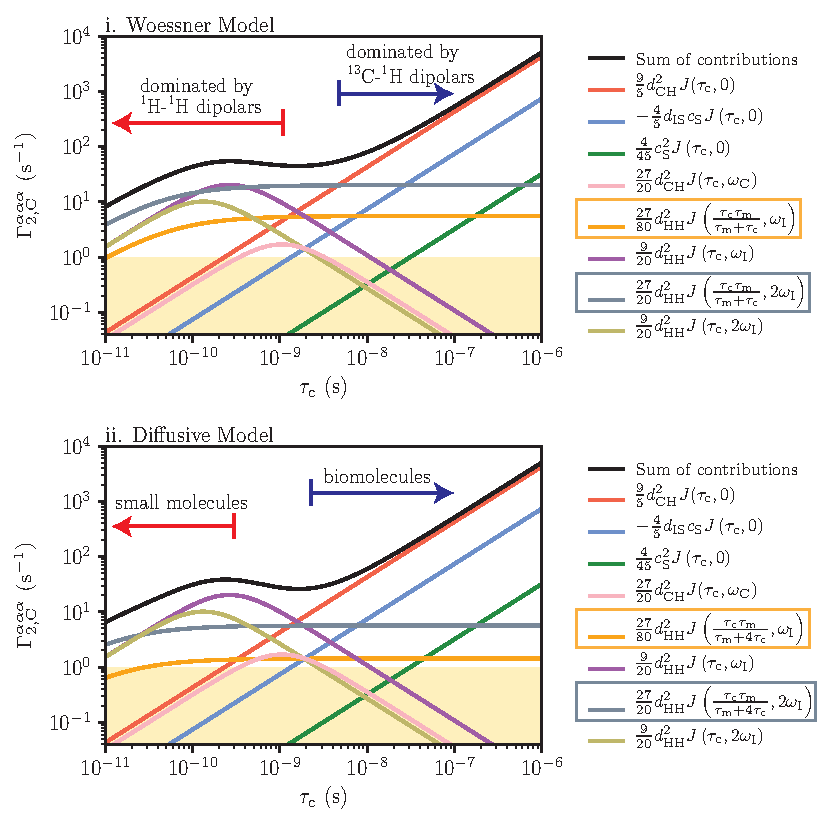
\includegraphics[scale=1]{./Figures/SimonsFigs/Contributions.pdf}
\caption{Plots of relaxation rate versus global tumbling correlation time, $\tau_{\text{c}}$, for the $\alpha \alpha \alpha$ peak in the $^{13}$C quartet (black lines), using the Woessner model (i.) and diffusive model (ii.). Individual terms in the rate expressions that contribute significantly over any range of $\tau_{\text{c}}$ are also plotted (coloured lines). All other terms reside within the yellow shaded region (or below the scale) for all $\tau_{\text{c}}$ values, and do not contribute to the rate in a significant manner in any region of the plot. The terms that cause differences between the two models are highlighted.}
\label{IndividualTerms}
\end{figure}
It is also in this region of the plot where the Diffusive and Woesssner models show the greatest deviations from each other. The lower rates predicted by the diffusive model are a result of the terms corresponding to the grey and orange lines in Figure \ref{IndividualTerms}. These terms are of a smaller magnitude when the diffusive model is considered, as they have spectral densities with $k_{\text{DW}} = 2$ associated with them. With the Woessner model, these terms have $k_{\text{DW}} = 1$ instead.\\
When larger values of $\tau_{\text{c}}$ are considered, the relaxation rates enter a linear regime, which corresponds to the macromolecular limit. This is since terms with spectral densities possessing frequency $0$ become dominant:
\begin{equation}
J(\tau_{\text{c}}, 0) = \tau_{\text{c}}
\end{equation}
For both the Diffusive and Woessner Models, the expressions for all four rates
collapse as follows, when only $J(\tau_{\text{c}}, 0)$ terms are considered:
\begin{equation}\label{MacroLim}
\begin{gathered}
\Gamma_{2,S}^{\alpha\alpha\alpha} \approx \frac{\tau_{\text{c}}}{45} \left( 9 d_{\text{IS}}^2  + 12 d_{\text{IS}} c_{\text{S}} + 4 c_{\text{S}}^2 \right) + \frac{3 \tau_{\text{c}} }{20} \sum \limits_i d_{\text{II},i}^2\\
\Gamma_{2,S}^{\alpha\alpha\beta} \approx \frac{\tau_{\text{c}}}{45} \left(d_{\text{IS}}^2  + 4 d_{\text{IS}} c_{\text{S}} + 4 c_{\text{S}}^2 \right) + \frac{3 \tau_{\text{c}}}{20} \sum \limits_i d_{\text{II},i}^2 \\
\Gamma_{2,S}^{\alpha\beta\beta} \approx \frac{\tau_{\text{c}}}{45} \left(d_{\text{IS}}^2  - 4 d_{\text{IS}} c_{\text{S}} + 4 c_{\text{S}}^2 \right) + \frac{3 \tau_{\text{c}} }{20} \sum \limits_i d_{\text{II},i}^2 \\
\Gamma_{2,S}^{\beta\beta\beta} \approx \frac{\tau_{\text{c}}}{45} \left(9 d_{\text{IS}}^2  - 12 d_{\text{IS}} c_{\text{S}} + 4 c_{\text{S}}^2 \right) + \frac{3 \tau_{\text{c}}}{20} \sum \limits_i d_{\text{II},i}^2
\end{gathered}
\end{equation}
From Figure \ref{IndividualTerms}, it is clear that the first term in these expressions, proportional to $d_{\text{IS}}^2$, is dominant in this limit, though $^{13}$C CSA contributions do also contribute to a noticeable extent.
\subsection{Summarising the Results}
The rate expressions presented by Ollerenshaw et al. are impressively accurate for methyl groups in molecules with large $\tau_{\text{c}}$ values, despite their simplicity relative to other models considered. This boils down to the fact that one particular term, arising from $^{13}$C-$^1$H dipolar interactions, dominates the relaxation behaviour in the macromolecular limit. Using fewer approximations, and crucially incorporating $^{13}$C CSA contributions, the model presented by Hansen et al. is highly accurate in the macromolecular limit. Their model and has been implemented in relaxation studies of methyls in proteins\cite{RN4}, indicating its validity. However, this model would be inadequate for calculations involving $^{13}$CF$_3$ moieties, since no consideration of the I-spin CSA is made. Whilst justifiable for methyl groups, where $\Delta \sigma_{\text{H}}$ is typically negligibly small, only models which include I-spin CSAs are likely to be appropriate for $^{13}$CF$_3$ studies.
\section{Comparing $^{13}$CH$_3$ with $^{13}$CF$_3$}
In order to gain a preliminary insight into the relative relaxation behaviour of $^{13}$CF$_3$ versus $^{13}$CH$_3$, the auto-relaxation rates of $^{13}$C single-quantum coherences were calculated. The results of these calculations are shown in Figure \ref{CvF}. It can be seen from these plots that all the relaxation rates are predicted to be lower for the trifluoromethyl moiety, relative to methyl, at all $\tau_{\text{c}}$ values. The $^{13}$CF$_3$ plots have been effectively translated down the $y$-axis slightly, relative to the $^{13}$CH$_3$ plots. This is of course highly promising from a TROSY perspective, where generating slowly relaxing magnetisations is the goal.\\
\begin{figure}
\centering
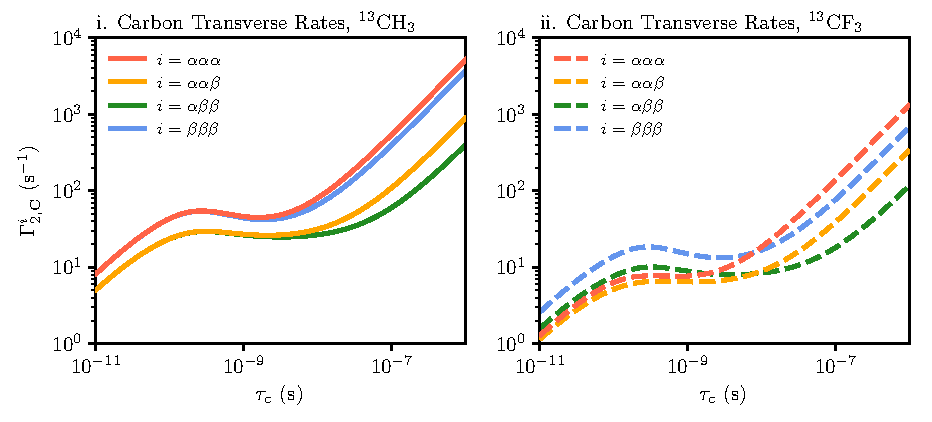
\includegraphics[scale=0.9]{./Figures/SimonsFigs/CvF.pdf}
\caption{Plots of transverse $^{13}$C relaxation rates versus global tumbling correlation time, $\tau_{\text{c}}$, for $^{13}$CH$_3$ and $^{13}$CF$_3$, using the Woessner Model. Parameters used: $B_0 = \num{14.1} \si{\tesla}$, $\gamma_{\text{C}} = \num{67.283e6} \si{\radian \per \second \per \tesla}$, $\gamma_{\text{H}} = \num{267.513e6} \si{\radian \per \second \per \tesla}$, $\gamma_{\text{F}} = \num{251.662e6} \si{\radian \per \second \per \tesla}$, $r_{\text{CH}} = r_{\text{HH}} = \num{1.09} \si{\angstrom}$, $r_{\text{CF}} = r_{\text{FF}} = \num{1.33} \si{\angstrom}$, $\beta = \ang{109.47}$, $\tau_{\text{m}} = \num{50} \si{\pico \second}$, $\Delta \sigma_{\text{C}} = \num{20} \text{ppm}$, $\Delta \sigma_{\text{H}} = \num{1} \text{ppm}$, $\Delta \sigma_{\text{F}} = \num{140} \text{ppm}$. A single external proton was considered, at an average distance of $\num{3} \si{\angstrom}$ from the $^1$H/$^{19}$F nuclei.}
\label{CvF}
\end{figure}
The major cause of the reduced $^{13}$CF$_3$ rates, relative to methyl is due to differences in dipolar couplings. The distances between the nuclei in the $^{13}$CF$_3$ moiety ($\num{1.33} \si{\angstrom}$) were set to be larger relative to the $^{13}$CH$_3$ distances ($\num{1.09} \si{\angstrom}$). Also, the gyromagnetic ratio of $^{19}$F is slightly smaller than that of $^1$H. These factors result in weaker dipolar interactions between the trifluoromethyl spins. The implication of these plots is that dipolar interactions are still the dominant relaxation-inducing mechanism in $^{13}$CF$_3$, despite the significantly elevated magnitude of the I-spin CSA. The impact of the $^{19}$F CSA should however be augmented as the magnetic field strength is increased\footnote{It can be seen from \ref{DipConst} and \ref{CSAConst} that $c_{\text{I}} \propto B_0$, whilst the dipolar constant, $d_{\text{IS}}$ has no dependence on $B_0$. Consequently, as $B_0$ is increased, the ratios $|\frac{c_{\text{I}}}{d_{\text{IS}}}|$ and $|\frac{c_{\text{I}}}{d_{\text{II}}}|$ will increase.}.
\subsection{Effect of Field Strength on $^{13}$CF$_3$ Rates}
NMR spectrometers operating at $^1$H Larmor frequencies of the order of gigahertz now exist, though these are not particularly commonplace at the time of writing. In order to assess the impact of higher field strengths on $^{13}$CF$_3$ relaxation rates, calculation ii. in Figure \ref{CvF} (corresponding to transverse $^{13}$C rates) was repeated, with $B_0$ set to $\num{23.49} \si{\tesla}$ (corresponding to a $\num{1} \si{\giga \myhertz}$ spectrometer).\\
\begin{figure}
\centering
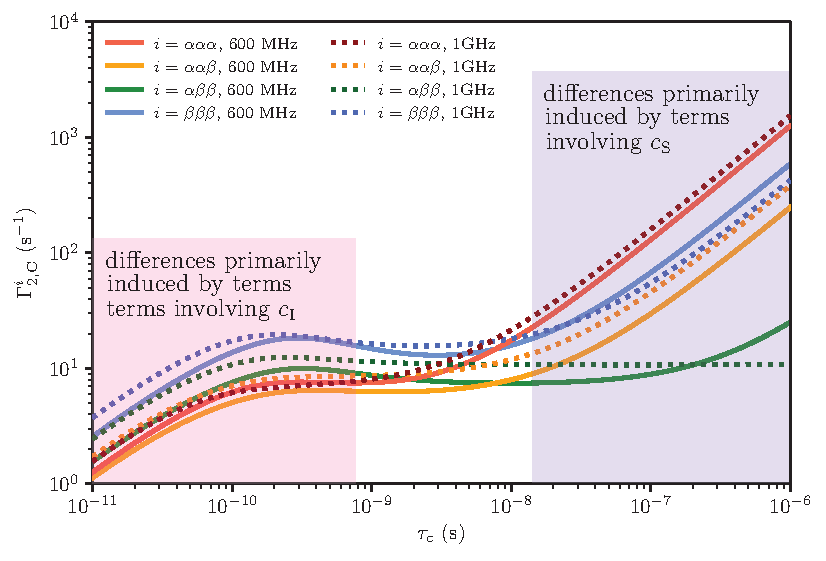
\includegraphics[scale=1]{./Figures/SimonsFigs/13CF3_1000.pdf}
\caption{Plots of $^{13}$C transverse relaxation rates, for a $^{13}$CF$_3$ moiety, using the Woessner Model. Two different field strengths were considered: $B_0 = \num{14.10} \si{\tesla}$ and $B_0 = \num{23.49} \si{\tesla}$, corresponding to $\num{600} \si{\mega \myhertz}$ and $\num{1} \si{\giga \myhertz}$ spectrometers, respectively. Parameters used: $\gamma_{\text{C}} = \num{67.283e6} \si{\radian \per \second \per \tesla}$, $\gamma_{\text{F}} = \num{251.662e6} \si{\radian \per \second \per \tesla}$, $r_{\text{CF}} = r_{\text{FF}} = \num{1.33} \si{\angstrom}$, $\theta = \ang{109.47}$, $\tau_{\text{m}} = \num{50} \si{\pico \second}$, $\Delta \sigma_{\text{C}} = \num{20} \text{ppm}$, $\Delta \sigma_{\text{F}} = \num{140} \text{ppm}$.}
\label{13CF3_1000}
\end{figure}
There are changes to all the relaxation rates when $B_0$ is increased, as can be seen in Figure \ref{13CF3_1000}. This indicates that chemical shift anisotropy effects are becoming more influential, as is to be expected. Yet even at the higher field strengths, dipolar effects are dominating the relaxation behaviour. Close inspection of the components in the rate expressions reveal that terms proportional to $c_{\text{I}}^2$ and $d_{\text{II}} c_{\text{I}}$ do have an impact on the rates when faster molecular tumbling is considered (i.e. small $\tau_{\text{c}}$). Despite this, as $\tau_{\text{c}}$ is increased, the impact of the $^{19}$F CSA becomes less significant. This is since none of the terms involving $c_{\text{I}}$ possess spectral densities with frequency $0$. The primary term causing the deviation in rate with field strength in the macromolecular limit is proportional to $d_{\text{IS}}c_{\text{S}} J\left(\tau_{\text{c}}, 0\right) = d_{\text{IS}}c_{\text{S}} \tau_{\text{c}}$. It is therefore the $^{13}$C CSA, coupled with the $^{13}$C-$^{19}$F dipolar interactions, that is driving the change in rates to the right hand side of Figure \ref{13CF3_1000}.\\
The calculations above indicate that the $^{19}$F CSA does not have a noticeable impact on $^{13}$C transverse relaxation rates in the macromolecular limit. Despite this, it may well be more influential when the relaxation of other coherences is considered. Any coherence for which the relaxation rate has a dependence on $A_1 A_2 J(\tau_{\text{c}},0)$, where $A_1$ and/or $A_2$ are $c_{\text{I}}$, is likely to be heavily influenced by the $^{19}$F CSA in the macromolecular limit. Significant deviations in behaviour relative to $^{13}$CH$_3$ systems are likely for such coherences, on top of the differences in dipolar contributions. Nevertheless, the calculations shown above provide strong evidence that the $^{13}$CF$_3$ moiety is likely to be an effective probe in an appropriate TROSY experiment, due to the low relaxation rates predicted relative to $^{13}$CH$_3$.
\subsection{The $\alpha \beta \beta$ Line}
The behaviour of the $\alpha \beta \beta$ line at high field strength deserves consideration. From Figure \ref{13CF3_1000}, the rate of this coherence plateaus in the macromolecular limit at sufficiently high field strength. The cause of this is an almost perfect cancellation of the terms in the expression for $\Gamma_{2,\text{S}}^{\alpha\beta\beta}$ (see Equation \ref{MacroLim}). This result already hints at a potential coherence that could be targeted via a $^{13}$CF$_3$ TROSY technique. Generation of $^{13}$C single quantum coherence, and subsequent selection of the $\alpha \beta \beta$ peak may well lead to highly intense spectra. Such selection processes exist, including a method introduced by Kontaxis and Bax\cite{RN3}.
